\cleardoublepage

\chapter{AVERAGING POWER DENSITY ON NONPLANAR SURFACES}
\label{chap:4}

\section{Normal Estimation on the Evaluation Surface}
\label{sec:normal_estimation_on_the_evaluation_surface}
The consideration of surface normals is fundamental in the computation of surface integrals of vector fields.
Namely, a vector field $\mathbf{v}$ on a surface $S$ results in a flux, given as the surface integral of the normal component of $\mathbf{v}$ over $S$.
As the tangential component of $\mathbf{v}$ does not contributes to the flux, it is disregarded by taking the dot product of $\mathbf{v}$ and the (unit) surface normal to $S$ at each point.
Thus, surface normals carry information on surface orientation by indicating the direction it faces relative to standard basis.
This information serves as a critical factor in accurately assessing the vector field flow across the surface.
It also allows vector fields to be appropriately spatially averaged on the surface which they pass through.
In general, a surface normal to a surface at a single point is represented by a vector perpendicular to the tangent plane at that particular point.

For any nonplanar surface $S$ in $\mathbb{R}^3$, parameterized by a system of curvilinear coordinates $u$ and $v$ as
\begin{align}
    \mathbf{r}(u, v) = \left( x(u, v), y(u, v), z(u, v) \right),
\end{align}
a normal to $S$ is given by 
\begin{align}
    \mathbf{n} = \frac{\partial \mathbf{r}}{\partial u} \times \frac{\partial \mathbf{r}}{\partial v}.
\end{align}

On the other hand, if a surface $S$ is instead given implicitly as $F(\mathbb{X}) = 0$ from an unorganized set of points $\mathbb{X} = \left\{ \mathbf{x}_1, \mathbf{x}_2, \dots, \mathbf{x}_n \right\} \subset \mathbb{R}^3$, a normal at a point $\mathbf{x}_i = (x_i, y_i, z_i) \in \mathbb{X}$, where $1 \leq i \leq n$, is given by
\begin{align}
    \mathbf{n} = \nabla F(\mathbb{X}),
\end{align}
since the gradient at any point is perpendicular to the level set $S$.

Finally, a surface $S$, given locally as the graph of a bi-variate ``height'' function relative to any $z$-direction that is not contained in the tangent plane, $z = f(x, y)$, is given as
\begin{align}
    \mathbf{r}(x, y) = \left( x, y, f \left( x, y \right) \right).
\end{align}
A surface normal is then defined as the cross product of partial derivatives of a ``height'' function,
\begin{align}
    \mathbf{n} = \frac{\partial \mathbf{r}}{\partial x} \times \frac{\partial \mathbf{r}}{\partial y}.
\end{align}
This way of assigning a surface normals is closely related to normals derived from the implicit surface form,
\begin{align}
    F(x, y, z) = z - f(x, y),
\end{align}
resulting in
\begin{align}
    \nabla F(x, y, z) = \left( -\frac{\partial f}{x}, -\frac{\partial f}{y}, 1 \right).
\end{align}
Here, it is assumed that a surface $S$ is smooth and continuously differentiable on a local scale (Lipschitz continuous).

\subsection{Normal Estimation on Nonplanar Canonical Surfaces}
It is fairly straightforward to determine the spatial distribution of surface normals to nonplanar canonical surfaces.
In differential geometry, a canonical surface refers to a class of surfaces that possess distinctive geometric properties allowing them to be defined by explicit expressions or parametric representations.
Two important nonplanar canonical surfaces, a sphere and a cylinder, are of special importance in human exposure to \gls{emf}s mostly because their shape matches the most exposed parts of the human body during practical exposure scenarios such as the head and finger, respectively.

Considering the ISO 80000-2:2019 convention~\cite{ISO2019Standard}, a sphere can be parameterized by using the spherical $(r, \theta, \varphi)$ coordinate system~\cite{Weisstein2023Spherical}.
Herein, $r$ represent the constant radial distance, i.e., the distance to origin. $\theta$ is the variable polar angle, and $\varphi$ is the variable angle of rotation from the initial meridian plane, i.e., azimuth angle.
From the parametric representation of the spherical surface,
\begin{align}
    \mathbf{r}(\theta, \varphi) = \left( r \sin\theta \cos\varphi, r \sin\theta \sin \varphi, r \cos\theta \right),
\end{align}
a surface normal is given by
\begin{align}
    \mathbf{n} = \frac{\mathbf{\partial r}}{\partial \theta} \times \frac{\mathbf{\partial r}}{\partial \varphi},
\end{align}
where $\nicefrac{\mathbf{\partial r}}{\partial \theta}$ and $\nicefrac{\mathbf{\partial r}}{\partial \varphi}$ are the partial derivatives of $\mathbf{r}$,
\begin{align}
    \frac{\mathbf{\partial r}}{\partial \theta} &= \left( r \cos\theta \cos\varphi, r \cos\theta \sin\varphi, -r \sin\varphi \right), \\
    \frac{\mathbf{\partial r}}{\partial \varphi} &= \left( -r \sin\theta \sin\varphi, r \sin\theta \cos\varphi, 0 \right),
\end{align}
and their magnitudes respectively correspond to
\begin{align}
    \left| \frac{\mathbf{\partial r}}{\partial \theta} \right| &= r,  \; \text{and}\\
    \left| \frac{\mathbf{\partial r}}{\partial \varphi} \right| &= r \sin\theta.
\end{align}
Thus, each surface normal is defined on the surface element spanning from $\theta$ to $\theta + \mathrm{d}\theta$ and from $\varphi$ to $\varphi + \mathrm{d}\varphi$,
\begin{align}
    \mathrm{d}S = \left\| \frac{\mathbf{\partial r}}{\partial \theta} \times \frac{\mathbf{\partial r}}{\partial \varphi} \right\| \mathrm{d}\theta \mathrm{d}\varphi = r^2 \sin\theta \; \mathrm{d}\theta \mathrm{d}\varphi.
\end{align}

On the other hand, considering the same convention~\cite{ISO2019Standard}, a cylinder is parameterized by using the cylindrical $(r, \theta, z)$ coordinate system~\cite{Sokolov2023Cylindrical}.
As in the case of a sphere, $r$ is treated as the constant radial distance and $\varphi$ represent the azimuth angle.
Additionally, $z$ represents the axial coordinate.
For this reason, a cylinder has zero Gaussian curvature, $K$, along its central axis.
On the other hand, a sphere is characterized by $K = \nicefrac{1}{r^2}$~\cite{Shikin2023Gaussian}.
Again, from the parametric representation of the cylindrical surface,
\begin{align}
    \mathbf{r}(\varphi, z) = \left( r \cos\varphi, r \sin \varphi, z \right),
\end{align}
a surface normal is given as
\begin{align}
    \mathbf{n} = \frac{\mathbf{\partial r}}{\partial \varphi} \times \frac{\mathbf{\partial r}}{\partial z},
\end{align}
where $\nicefrac{\mathbf{\partial r}}{\partial \varphi}$ and $\nicefrac{\mathbf{\partial r}}{\partial z}$ are the partial derivatives of $\mathbf{r}$,
\begin{align}
    \frac{\mathbf{\partial r}}{\partial \varphi} &= \left( -r \sin\varphi, r \cos\varphi, 0 \right), \\
    \frac{\mathbf{\partial r}}{\partial z} &= \left( 0, 0, 1 \right),
\end{align}
and their magnitudes respectively correspond to
\begin{align}
    \left| \frac{\mathbf{\partial r}}{\partial \varphi} \right| &= r, \; \text{and}\\
    \left| \frac{\mathbf{\partial r}}{\partial z} \right| &= 1.
\end{align}
The surface element spanning from $\varphi$ to $\varphi + \mathrm{d}\varphi$ and from $z$ to $z + \mathrm{d}z$ is given as
\begin{align}
    \mathrm{d}S = \left\| \frac{\mathbf{\partial r}}{\partial \varphi} \times \frac{\mathbf{\partial r}}{\partial z} \right\| \mathrm{d}\varphi \mathrm{d}z = r \; \mathrm{d}\varphi \mathrm{d}z.
\end{align}

Contrary to surface normals whose magnitude represents the local curvature of a surface at a particular point, a unit normal is the Euclidean vector of unit length.
It represents the direction vector,
\begin{align}
    \mathbf{\hat n} = \frac{\mathbf{n}}{\left| \mathbf{n} \right|},
\end{align}
where $\left| \mathbf{n} \right|$ is the vector norm of $\mathbf{n}$~\cite{Weisstein2023Unit}.
The spatial distribution of unit normals to the sphere and lateral surface of the cylinder is shown respectively in panel \textbf{a} and \textbf{b} in~\cref{fig:normals}.
Herein, unit normal vectors are mapped into corresponding \gls{rgb} value based on the \gls{rgb} color space represented by the \gls{rgb} cube, shown in panel \textbf{c} in~\cref{fig:normals}.
Each component of a unit normal ($x$, $y$, and $z$) is transformed into the corresponding color channel (red, green, and blue).
\begin{figure}[t]
    \centering
    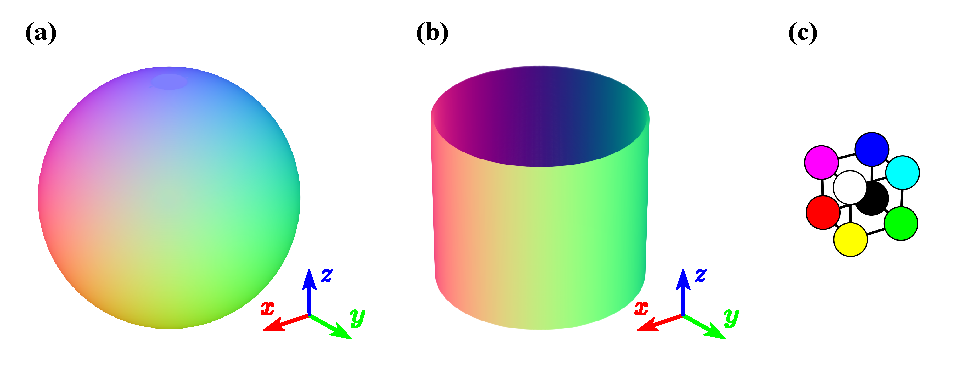
\includegraphics[width=0.96\textwidth]{artwork/normals.pdf}
    \caption{Spatial distribution of unit normal vectors on (a) the sphere and (b) lateral surface of the cylinder, represented by red-green-blue values with respect to (c) the color cube.}
    \label{fig:normals}
\end{figure}

\subsection{Normal Estimation on Nonplanar Anatomical Surfaces}
Anatomical body models are usually created as either the computer-aided design or voxel computational models.
These models are developed upon medical scans and images to a certain level of resolution, which is dependent on the resolution of recording devices.
A very efficient representation of an anatomical model is by using the unstructured \gls{3-d} point cloud on the surface.
The surface of a model represents a compact, connected and orientable \gls{2-d} manifold embedded in $\mathbb{R}^3$.
A point cloud on the surface is represented as a collection of coordinates $\mathbb{X} = \left\{ \mathbf{x}_1, \mathbf{x}_2, \dots, \mathbf{x}_n \right\}$ where $\mathbf{x}_i = (x_i, y_i, z_i) \in \mathbb{X}, \; 1 \leq i \leq n$.

If the model itself does not contain any information on surface normals, they should be estimated at every point in the iterative manner on a local scale~\cite{Berger2017survey}.
There are several existing normal estimation techniques, each adapted according to the particular shape of the surface, noise level, the incidence of sharp edges, etc.
These techniques are broadly classified into two separate classes: ``traditional'' and learning-based normal estimation.

``Traditional'' techniques generally rely on the analysis of the covariance matrix composed from a local patch around a query point in the cloud.
Furthermore, these techniques can be divided into two additional sub-classes: optimization-based and averaging techniques~\cite{Klasing2009Comparison}.
Optimization-based techniques estimate a normal by minimizing the cost function penalizing a certain criterion, such as the distance of points to a local tangent plane or the angle between tangential vectors and the normal vector~\cite{Hoppe1992Surface}.
On the contrary, averaging techniques are calculating the normal vector as the weighted average of normal vectors on the triangles formed with pairs of neighboring points within a local patch~\cite{Jin2005comparison}.

Learning-based techniques are divided into the regression- and surface fitting-based techniques~\cite{Wang2015Designing}.
These techniques are introduced in order to solve recurrent issues in normal estimation on non-differentiable/non-smooth regions on the surface.
In addition, learning-based techniques significantly improve robustness to various noise levels and point density variations.
Regression-based techniques directly predict the direction of each normal utilizing various architectures of deep neural networks and the latest achievements in computer vision research~\cite{Charles2017PointNet,Guerrero2018PCPNet,Ben-Shabat2019Nesti-Net,Zhou2023Refine-Net}.
Surface fitting-based techniques effectively act as an extension to any ``traditional'' technique.
In most cases this involves using deep neural networks to predict the optimal set of weights either for the tangent plane fitting or extraction of the local neighborhood around a query point~\cite{Lenssen2020Deep,Ben-Shabat2020DeepFit,Zhu2021AdaFit,Li2022HSurf-Net}.

Given the anatomical models are generally free of noise and outliers, sampled densely enough, and differentiable across the entire surface, the focus in this thesis is on ``traditional'' techniques, primarily on techniques based on (weighted) moving least squares, which will be discussed in more detail later in the chapter.

A unit normal vector, $\mathbf{\hat n}$, is assigned at each point, $\mathbf{x}_i$, of the point cloud, $\mathbb{X}$.
The direction of $\mathbf{\hat n}$ is estimated by fitting a local plane and extracting its principal components.
First, $\mathbb{X}$ is organized into a \gls{k-d} tree, a space-partitioning data structure that allows searching for the nearest neighbors of a point according to a certain criterion~\cite{Bentley1975Multidimensional}.
Then, $k$ nearest neighbors around $\mathbf{x}_i$ are extracted.
The nearest neighbors represent a local patch of points, $nbhd(\mathbf{x}_i)$, from which the covariance matrix is composed.
After decomposition of the matrix by using the \gls{pca}, the eigenvector with the smallest corresponding eigenvalue is orthogonal to the tangent plane at $\mathbf{x}_i$ and thus represents the unit normal vector.
Other two eigenvectors lie in the tangent plane and represent the unit binormal, $\mathbf{\hat b}$, and unit tangent vector, $\mathbf{\hat t}$.
In the illustrative example shown in~\cref{fig:normal_estimation}, a positional relationship between principal components extracted from the covariance matrix of $nbhd(\mathbf{x}_i)$ is shown.
\begin{figure}[t]
    \centering
    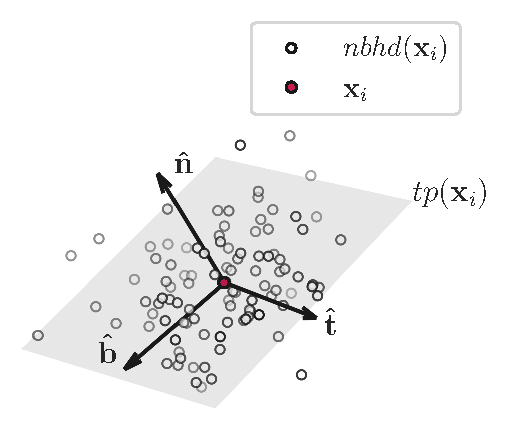
\includegraphics[width=0.46\textwidth]{artwork/normal_estimation.pdf}
    \caption{The unit binormal, tangent and normal vector at the query point with respect to the local neighborhood surrounding that point.}
    \label{fig:normal_estimation}
\end{figure}
These three orthogonal vectors $\left\{ \mathbf{\hat b}, \mathbf{\hat t}, \mathbf{\hat n} \right\}$ span $\mathbb{R}^3$ and form an orthonormal basis on a local scale with $\mathbf{x}_i$ at the origin.
This process should be repeated for each $\mathbf{x}_i$ in $\mathbb{X}$ to obtain the unit normal vector field over the entire surface.

Fitting a local tangent plane to a query point is performed as follows.
The ``centroid'' of $nbhd(\mathbf{x}_i)$ is first computed as
\begin{align}
    m_i = \frac{1}{k} \; \sum_{j=1}^{k} \mathbf{x}_j.
\end{align}
Here, $k$ stands for the number of points in $nbhd(\mathbf{x}_i)$, whereas $\mathbf{x}_j$ represents a point in $nbhd(\mathbf{x}_i)$.
A tangential plane can then be found by minimizing the Euclidean distance vector, $\mathbf{y}_j$, between each point in $nbhd(\mathbf{x}_i)$ and $\mathbf{m}_i$
\begin{align}
    \label{eqn:constrained_1}
    \min_{\left| \mathbf{n}_i \right| = 1} \sum_{j=1}^{k} \left( \mathbf{y}_j^\intercal \mathbf{n}_i \right)^2.
\end{align}
The above expression can be rewritten in matrix notation as
\begin{align}
    \label{eqn:constrained_2}
    \min_{ \mathbf{n}_i^\intercal \mathbf{n}_i = 1} \mathbf{n}_i^\intercal \left( \mathbf{Y}_i \mathbf{Y}_i^\intercal \right) \mathbf{n}_i,
\end{align}
where
\begin{align}
    \mathbf{Y}_i = \begin{pmatrix}
    \vline & \vline &  & \vline &  & \vline \\
    \mathbf{y}_1 & \mathbf{y}_2 & \dots & \mathbf{y}_j & \dots & \mathbf{y}_k \\
    \vline & \vline &  & \vline &  & \vline
    \end{pmatrix}.
\end{align}

Instead of the imposed constrained optimization in~\cref{eqn:constrained_1,eqn:constrained_2}, $f(\mathbf{n}_i) = \mathbf{n}_i^\intercal \mathbf{S}_i \mathbf{n}_i$, where $\mathbf{S}_i = \mathbf{Y}_i \mathbf{Y}_i^\intercal$, is subjected to the equality constraint, $g(\mathbf{n}_i) = \mathbf{n}_i^\intercal \mathbf{n}_i - 1$, and the Lagrangian function is constructed as
\begin{equation*}
    \mathcal{L}(\mathbf{n}_i, \lambda) = f(\mathbf{n}_i) - \lambda g(\mathbf{n}_i).
\end{equation*}
The constrained optimization is now converted into the unconstrained minimization of $\mathcal{L}(\mathbf{n}_i, \lambda)$ simply by equating the gradient of the Lagrangian to zero,
\begin{align}
    \nabla \mathcal{L}(\mathbf{n}_i, \lambda) &= 0, \\
    \frac{\partial \mathcal{L}}{\partial \mathbf{n}_i} &= 0 \Rightarrow \mathbf{S}_i \mathbf{n}_i = \lambda \mathbf{n}_i, \\
    \frac{\partial \mathcal{L}}{\partial \lambda} &= 0 \Rightarrow \mathbf{n}_i^\intercal \mathbf{n}_i = 1.
\end{align}
A (unit) normal is then captured from
\begin{align}
    \mathbf{S}_i = \mathbf{V} \begin{pmatrix}
    \lambda_1 &  &  \\
    & \ddots & \\
    & & \lambda_d
    \end{pmatrix} \boldsymbol{V}^\intercal
\end{align}
as the eigenvector with the smallest corresponding eigenvalue.

Instead of a plane, a higher-order polynomial~\cite{Levin1998approximation}, implicit B-spline~\cite{Rouhani2015Implicit} and osculating jets (truncated Taylor expansion)~\cite{Cazals2005Estimating} can be fitted to a parametric surface in orthonormal basis.   
This is particularly important when surface normals, rather than unit normals, should be determined.
In such cases, a surface (or curvature) normal is computed as
\begin{align}
    \mathbf{n} = \frac{\partial \tilde f}{\partial u} \times \frac{\partial \tilde f}{\partial v}
\end{align}
at tangential coordinates $u = v = 0$ where $\tilde{f}(u, v)$ is the fitted ``height'' function in the normal direction.

Generally, the approach in normal estimation described previously will certainly lead to inconsistent orientation of the unit normal vector field on the surface.
This is mainly due to eigenvectors being arbitrarily oriented due to the computer implantation of the numerical solver used for the eigendecomposition of the covariance matrix.
The issue of inconsistent orientation can be resolved by finding a consistent global orientation by propagation starting from a certain viewpoint.
In general, for $\mathbb{X}$ of sufficient density given that the surface is differentiable, adjacent normal vectors, $\mathbf{n}_i$ and $\mathbf{n}_j$, at any two neighboring points, $\mathbf{x}_i$ and $\mathbf{x}_j$, should point in a similar direction.
In other words, $\mathbf{n}_i \cdot \mathbf{n}_j \approx \pm 1$ if corresponding tangent planes $tp(\mathbf{x}_i)$ and $tp(\mathbf{x}_j)$ are (nearly) parallel.
If the planes are consistently oriented then $\mathbf{n}_i \cdot \mathbf{n}_j \approx 1$.
Otherwise, if $\mathbf{n}_i \cdot \mathbf{n}_j \approx -1$, either $\mathbf{n}_i$ or $\mathbf{n}_j$ must be flipped.

This approach has two main disadvantages: it fails at sharp edges and corners, and the imposed condition should hold for \emph{all} pairs of neighboring points in the point cloud.
Since anatomical tissue models do not contain sharp edges and corners, the first outlined disadvantage can be disregarded.
Furthermore, the second shortcoming can be taken care of by constructing a so called Riemann graph over the point cloud and assigning a weight to each edge based on the similarity score between the respective points' normals~\cite{Hoppe1992Surface},
\begin{align}
    w_{ij} = 1 - \left| \mathbf{n}_i \cdot \mathbf{n}_j \right|
\end{align}
This allows the construction a minimal spanning tree across which the initial normal orientation from a single point selected as the root can be efficiently propagated.
The favorable propagation is the one that follows the direction of low curvature, thereby avoiding ambiguous situations~\cite{Berger2017survey}.

In~\cref{fig:normals_ear}, the spatial distribution of surface normals on the surface of the adult ear model is shown.
This model is taken from the third published study highlighted in~\cref{sec:publication_3}.
Surface normals are first normalized to unit length and then mapped into corresponding \gls{rgb} values (the frame of reference is shown in lower right region in~\cref{fig:normals_ear}).
\begin{figure}[t]
    \centering
    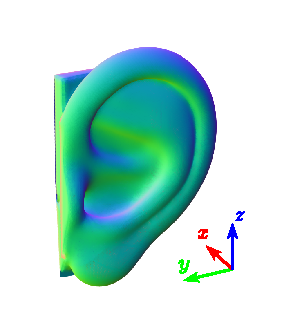
\includegraphics[width=0.4\textwidth]{artwork/normals.ear.pdf}
    \caption{Spatial distribution of normal vectors on the surface of the ear model represented by red-green-blue values.}
    \label{fig:normals_ear}
\end{figure}

\section{Construction of the Averaging Area}
\label{sec:construction_of_the_averaging_area}
The spatially averaged power density is acquired through the computation of surface integrals over the conformal averaging area, $\hat A$, on the evaluation surface.
The extent of this averaging area is contingent upon the configuration of the evaluation surface itself within the computational domain.
In the case of a nonplanar evaluation surface, the averaging area surpasses the size of its \gls{2-d} projection.
Conversely, if the evaluation surface is flat, the averaging area corresponds to the square-shape averaging area of \SIlist{4;1}{\cm\squared} as prescribed in~\cite{ICNIRP2020Guidelines,IEEE2019Standard}.

In the case of evaluation surfaces that are entirely flat, the construction of the averaging area is straightforward.
For a \SI{4}{\cm\squared} averaging area, a square shape with an edge length of \SI{2}{\cm} is employed, whereas a \SI{1}{\cm\squared} averaging area is represented by a square with an edge length of \SI{1}{\cm}~\cite{IEEE2021Guide}.
The positioning of the averaging area on the evaluation surface is determined by its center point, which corresponds to the intersection of the diagonals of the square.
To ascertain the orientation that maximizes the power passing through the averaging area, the square is rotated around its center point in increments of up to \SI{5}{\degree}~\cite{IEC63195-2-2022}.
The maximum spatially averaged power density with regards to the relative orientation at a query point is determined; further information regarding the integration of power density can be found in~\cref{sec:spatial_averaging_of_power_density}.
This process is repeated for all points on the evaluation surface.
The peak spatial-averaged power density is then reported at the point, which results in a global maximum of the spatially averaged power density.

The averaging area on the nonplanar evaluation surface is determined as the intersection with a sphere of a fixed size defined by radius $r_\text{av}$; panel \textbf{a} in~\cref{fig:evaluation_surface}.
\begin{figure}[t]
    \centering
    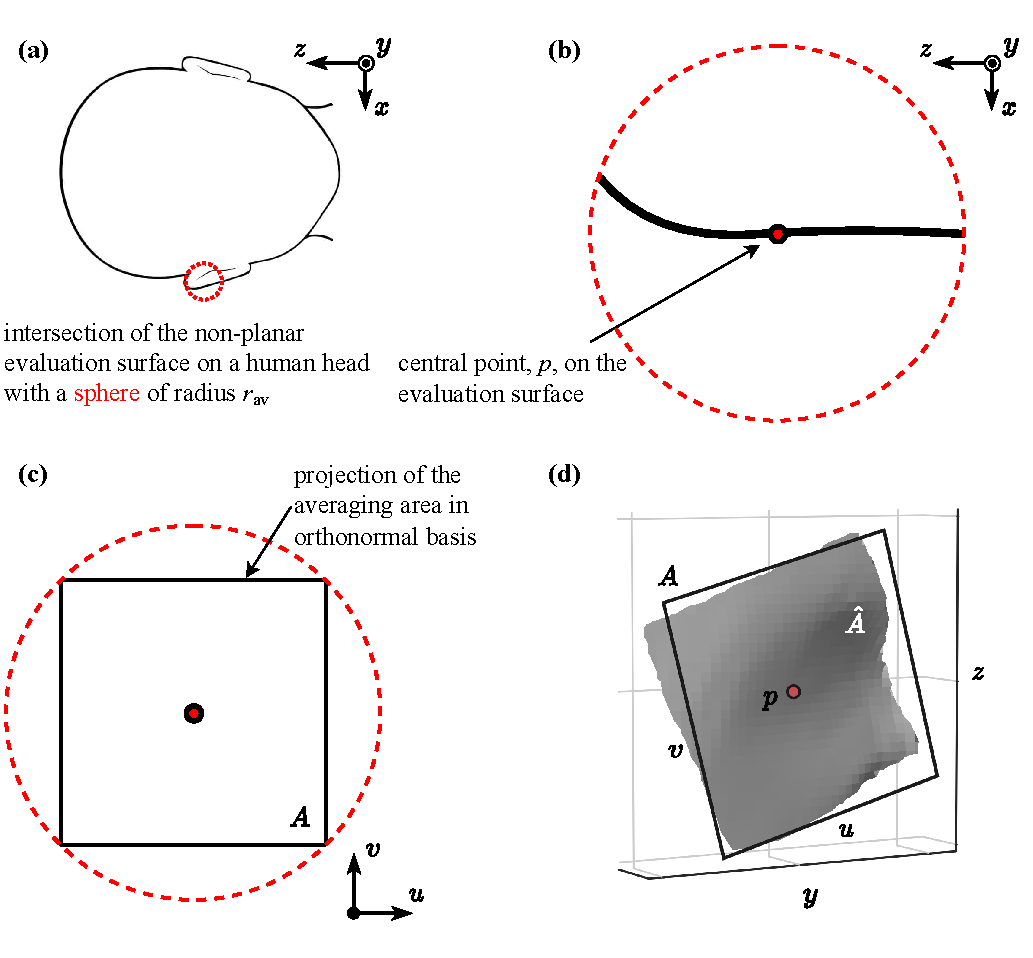
\includegraphics[width=\textwidth]{artwork/evaluation_surface.pdf}
    \caption{Construction of the averaging area on a nonplanar evaluation surface: (a) intersection of the surface of the human head with a sphere of fixed radius, (b) position of the center point of the sphere at the evaluation surface, (c) projection of the averaging area in two-dimensional space, (d) spatial relationship between the conformal averaging area and its projection.}
    \label{fig:evaluation_surface}
\end{figure}
Contrary to recommendations in~\cite{IEC63195-2-2022}, the radius is here defined as
\begin{align}
    r_\text{av} = \frac{\sqrt{2 A}}{2},
\end{align}
where $A$ is the square-shape flat averaging area.
Thus, $r_\text{av}$ corresponds to the radius of the circumscribed circle of the square-shape averaging area.
In general, a circumscribed circle (circumcircle) of a polygon is a circle that passes through all the vertices of that polygon.
The center point of a sphere is a point on the evaluation surface, shown in panel \textbf{b} in~\cref{fig:evaluation_surface}.

The averaging area is then reduced to match square shape in an orthonormal basis as follows.
First, a local patch of points contained in the intersected region is centered at zero-mean by computing the average of $x$, $y$ and $z$ coordinates and subtracting it from each point.
Subsequently, the covariance matrix is computed based on these centered coordinates.
The eigenvectors associated with the two largest eigenvalues are then identified as they represent the primary directions of variance in the spatial distribution of coordinates when projected in \gls{2-d} space.
These selected eigenvectors serve as the columns of a transformation matrix.
By multiplying the centered point cloud with this transformation matrix, it is effectively represented in \gls{2-d} space defined by parametric coordinates $u$ and $v$.
Finally, the resulting projection is constrained to match the shape and dimensions of the square-shape averaging area, $A$, of \SIlist{4;1}{\cm\squared}, as illustrated in panel \textbf{c} in~\cref{fig:evaluation_surface}.

Once the square-shape projection is transformed back into standard basis, the conformal averaging area, $\hat A$, is obtained (panel \textbf{d} in~\cref{fig:evaluation_surface}).
Due to the nonplanar shape of the evaluation surface, the area $\hat A$ is greater than $A$.
This deviation in size is influenced by the degree of curvature present on the evaluation surface, adhering to the principle: the greater the curvature, the greater the overall difference.
Nonetheless, by transforming the original intersection into \gls{2-d} space defined by its principal components, it is ensured that this deviation is minimized.

The method of assessment of the conformal averaging area depends on the surface discretization within the computational domain.
For example, if the evaluation surface is discretized by using triangle mesh, the standardized algorithm for area estimation exists~\cite{IEC63195-2-2022}:
\begin{itemize}
    \item specify an empty list of triangles;
    \item determine the triangles on the evaluation surface that are completely enclosed within a region of the bounded conformal averaging area;
    \item append the encompassed triangles to the list of triangles specified in the first step that are connected to the triangles that contain the center point via other triangles that are located completely inside a region of the bounded conformal averaging area;
    \item determine the triangles that intersect the surface of the sphere and the intersection points of their edges with the averaging surface; determine the triangles specified by these intersection points and the corner points of the triangles of the evaluation surface; if the geometric centers of the triangles are inside the averaging surface, add the triangles to the list;
    \item sum the areas of all triangles contained in the list.
\end{itemize}

Alternatively, when solely the spatial distribution of unstructured points sampled on the surface is available, without any information about the positional relationship between the points, the conformal averaging area can be estimated by approximating the surface integral of the magnitude of the surface normal vector field.
The surface integral is precisely defined within the bounds of the parameters. 
These parameter bounds are determined to represent the surface as a graph of a bi-variate ``height'' function, relative to the $z$-direction aligned with the unit normal at the center point on that surface.
This approach guarantees the square shape of the integration domain and the magnitude of surface normals is represented as the scalar field on this integration domain as
\begin{align}
    \left| \mathbf{\tilde n} \right| = f(x, y).
\end{align}
The integral can be approximated by any accurate \gls{2-d} quadrature technique.
One approach is to fit the scalar field by a smooth bi-variate spline constructed as tensor products of \gls{1-d} splines to satisfy
\begin{align}
    \sum_{i} \left[ w_i \left( f(x_i, y_i) - \left| \mathbf{n}_i \right| \right) \right]^2 \leq s,
\end{align}
where $w_i$ are non-negative weights, and $s$ is the smoothing factor, which controls the smoothness of the resulting function $f(x, y)$ and the overall accuracy of the approximation. 
\Gls{1-d} splines are defined by the specific polynomial degree separately in $x$- and $y$-direction.
Generally, for data sampled densely enough, a bi-cubic spline is a natural choice.
As the integral of a bi-cubic spline can be calculated analytically, the surface integral of $f(x, y)$ is determined as the incremental sum of contributions of individual splines within the integration domain on which $f(x, y)$ is defined.

\section{Spatial Averaging of Power Density}
\label{sec:spatial_averaging_of_power_density}
In practical applications, compliance with the current exposure limits at \SIrange{6}{300}{\GHz} involves the computation of spatially averaged \gls{ipd}.
The spatially averaged \gls{ipd} on the surface of the exposed tissue is subject to various specifications, which depend on the prevailing incidence direction and polarization of the \gls{emf}~\cite{IEC63195-2-2022}.
The integrand functions corresponding to these specification are multiplied by additional functions that account for the angle between the Poynting vector and surface normals.
This ensures that contributions from regions where the Poynting vector points outward from the evaluation surface or is parallel to the tangential plane at a specific point on the surface are not considered in computation.

The first specification pertains to the power density of the surface-normal propagation direction into the evaluation surface.
The computation of the spatially averaged power density at a specific location, as determined by the position vector, $\mathbf{r}_0$, follows the expression presented below~\cite{IEC63195-2-2022}:
\begin{align}
    \label{eqn:propagation-direction}
    S_\text{inc, n}(\mathbf{r}_0) = \frac{1}{2 \hat{A}\left( \mathbf{r}_0 \right)} \; \iint_{A \left( \mathbf{r}_0 \right)} \Theta \left\{ \Re \left[ \mathbf{E \left( r \right)} \times \mathbf{H^* \left( r \right)} \right] \cdot \mathbf{\hat{n} \left( r \right)} \right\} \cdot \Re \left[ \mathbf{E \left( r \right)} \times \mathbf{H^* \left( r \right)} \right] \cdot \mathbf{\hat{n} \left( r \right)} \; \mathrm{d}\hat{A}\left( \mathbf{r} \right).
\end{align}
In this equation, the Heaviside function, $\Theta(\cdot)$, assumes a crucial role.
This function ensures that the integrand function is zero if the angle between the Poynting vector and a normal vector (which is assumed to point into the irradiated solid volume bounded by the surface) is within the \SIrange{90}{270}{\degree} range.
This adjustment is necessary to account for situations where the normal component of the Poynting vector would otherwise yield a negative value.
Additionally, within the equation, $\hat A$ stands for the conformal averaging area, with $\hat A$ being always greater than $A$ for nonplanar surfaces.
The positional vector, denoted as $\mathbf{r}$, refers to a point on the surface determined by the area $\hat A$.

Additionally, the total propagating power density into the evaluation surface, is defined in~\cite{IEC63195-1-2022,IEC63195-2-2022} as
\begin{align}
    \label{eqn:total}
    S_\text{inc, tot}(\mathbf{r}_0) = \frac{1}{2 \hat{A}(\mathbf{r}_0)} \iint_{A(\mathbf{r}_0)} \left\| \Re \left[ \mathbf{E}(\mathbf{r}) \times \mathbf{H}^*(\mathbf{r}) \right] \right\| \cdot \Xi \left( \delta \right) \; \mathrm{d}\hat{A}(\mathbf{r}),
\end{align}
where
\begin{align}
    \delta = \cos^{-1}\left[ {\frac{\Re \left[ \mathbf{E}(\mathbf{r}) \times \mathbf{H}(\mathbf{r})^* \right]}{\left\| \Re \left[ \mathbf{E}(\mathbf{r}) \times \mathbf{H}(\mathbf{r})^* \right] \right\|} \cdot \mathbf{n}(\mathbf{r})} \right],
\end{align}
and
\begin{align}
\Xi(\delta) = \begin{cases}
        1, & \text{if } \SI{0}{\degree} \leq \delta < \SI{85}{\degree} \\
        1 - \nicefrac{(\delta - \SI{85}{\degree})}{\SI{5}{\degree}}, & \text{if } \SI{85}{\degree} \leq \delta < \SI{90}{\degree} \\
        0, & \text{otherwise}.
    \end{cases}
\end{align}

The final aspect to note is the exclusion of the discussion on the total power density directed into the exposed model in the context of near-field exposure.
Specifically, in the reactive near field, the prevailing influence stems from the non-propagating energy encapsulated within the imaginary component of the Poynting vector.
Consequently, the magnitude of the imaginary part should be incorporated into the spatial averaging procedure.
However, it is important to highlight that both the \gls{icnirp} guidelines~\cite{ICNIRP2020Guidelines} and \gls{ieee} standard~\cite{IEEE2019Standard} advise against assessment of the spatially averaged \gls{ipd} in the reactive near field.
Instead, in this region, the determination of \gls{br}s is recommended as the appropriate approach.

Any accurate \gls{2-d} quadrature technique may be employed in order to solve for surface integrals specified in~\cref{eqn:propagation-direction,eqn:total}.
In most cases, the choice of the quadrature method depends on the interpolation approach adopted for the integrand function.
In general, the Gauss-Kronrod quadrature formula, can be utilized regardless of the interpolation method employed.
This adaptive numerical integration method is based on Gaussian quadrature, with evaluation points selected strategically to ensure an accurate approximation by utilizing information obtained from computations of less accurate approximations.
Furthermore, this method eliminates the need for explicitly defining the degree of quadrature.
A typical choice combines a \num{7}-point Gauss rule with a \num{15}-point Kronrod rule~\cite{Kahaner1989Numerical}.
However, it is important to note that the Gauss-Kronrod quadrature can be computationally intensive, particularly when a large number of surface integrals needs to be evaluated, depending on the complexity of the integrand function.
A detailed discussion on the selection of the quadrature technique can be found in the fourth published paper in~\cref{sec:publication_4}.

The automatic detection of the region of highest exposure involves a set of sequential steps, as outlined below:
\begin{itemize}
    \item assuming a nonplanar model is represented by an oriented set of points $\mathbb{X} = \{ \mathbf{x}_1, \mathbf{x}_2, \dots, \mathbf{x}_n \} \subset \mathbb{R}^3$, organize it into a \gls{3-d} \gls{k-d} tree;
    \item identify points visible from the predefined direction~\cite{Katz2007Direct}, which should correspond to the propagation direction of the \gls{emf}; this step is optional, but it allows to focus solely on a region that is in the line of sight of \gls{emf} sources;
    \item for each point (in the visible subset of points), extract the local neighborhood by considering points located within a sphere of a radius $\nicefrac{\sqrt{2 A}}{2}$, where $A$ represents the size of the square integration domain;
    \item perform a change of basis on the local neighborhood using the \gls{pca}, which leads to the alignment of the tangential principal components with $A$;
    \item compute the area of a conformal averaging area, $\hat A$, by approximating the surface integral of the magnitude of surface normals on the corresponding surface;
    \item compute the spatially averaged power density using the approach outlined in~\cref{eqn:propagation-direction,eqn:total}.
\end{itemize} 

To demonstrate the practical application of the automated detection, we consider the realistic human head model\footnote{Courtesy of H. Dodig, University of Split, Faculty of Maritime Studies} exposed to \gls{rf} energy in a Gaussian pattern~\cite{Foster2016Thermal} (approximating the exposure conditions in~\cite{Colombi2015Implications}).
The original \gls{3-d} model is constructed from magnetic resonance imaging scans of a \num{24}-year-old male volunteer~\cite{Laakso2015Intersubject}.
However, in this illustration, we represent the input model as an unstructured point cloud comprising \num{63333} surface points.
The reconstructed surface of the point cloud model, obtained using the Poisson method~\cite{Kazhdan2006Poisson}, which solves for an approximate indicator function matching the input normals' gradient, is depicted in panel \textbf{a} in~\cref{fig:head}.

The estimation of surface normals is carried out by using the weighted least squares method~\cite{Levin1998approximation}, as outlined in the preceding section.
The spatial distribution of unit normals on the surface of the head model is visualized in panel \textbf{b} in~\cref{fig:head}, using the \gls{rgb} representation.
It is important to note that the surface normals are shown pointing outward from the volume enclosed by the surface.
However, during subsequent spatial averaging of the power density, the normals are assumed to point inward to align with the direction of incidence of the \gls{emf}, thereby avoiding any physical inconsistencies.

The power density incident on the surface of the human head follows a Gaussian pattern, depicted in panel \textbf{c} in~\cref{fig:head} and mathematically represented by the following expression:
\begin{align}
    S_\text{inc}(x, y, z) = I_0 \; e^{-\left( \nicefrac{d}{\rho} \right)^2}.
\end{align}
In the equation, $I_0$ represents the peak \gls{ipd} of \SI{10}{\watt\per\m\squared}, located at the point closest to the theoretical radiation source with respect to the $x$-axis in the upper crus region of the antihelix on the right outer ear.
The scaled Euclidean distance, here denoted by $d$, measures the distance between the point of the peak \gls{ipd}, $(x_c, y_c, z_c)$, and a point on the evaluation surface, $(x, y, z)$.
The original Euclidean distance is additionally scaled to deform the otherwise circular pattern into an elliptical shape as
\begin{align}
    d = d(x, y, z) = \sqrt{\left( \frac{(x - x_c)^2}{s_x} + \frac{(y - y_c)^2}{s_y} + \frac{(z - z_c)^2}{s_z} \right)},
\end{align}
where  $s_x$, $s_y$ and $s_z$ correspond to \num{1}, \num{0.5} and \num{0.25}, respectively.
The scaled distance is bounded within the radius of ``influence'', $\rho$, set to \SI{2.5}{\cm} in this particular case.

Finally, panel \textbf{d} in~\cref{fig:head} shows the square projection of the conformal averaging area corresponding to the most exposed region on the evaluation surface.
Before executing the algorithm for automated detection of the peak spatial-averaged power density, the surface is resampled into a point cloud where only the points directly visible from the perspective of the \gls{emf} incidence point of view (in the negative $x$-direction) are considered.
The hidden point removal operator~\cite{Katz2007Direct}, which determines the visible points in a point cloud, as viewed from any given viewpoint is employed.
The spatial averaging of the power density within this region of the surface yields a value of \SI{4.45}{\watt\per\m\squared}.
\begin{figure}[t]
    \centering
    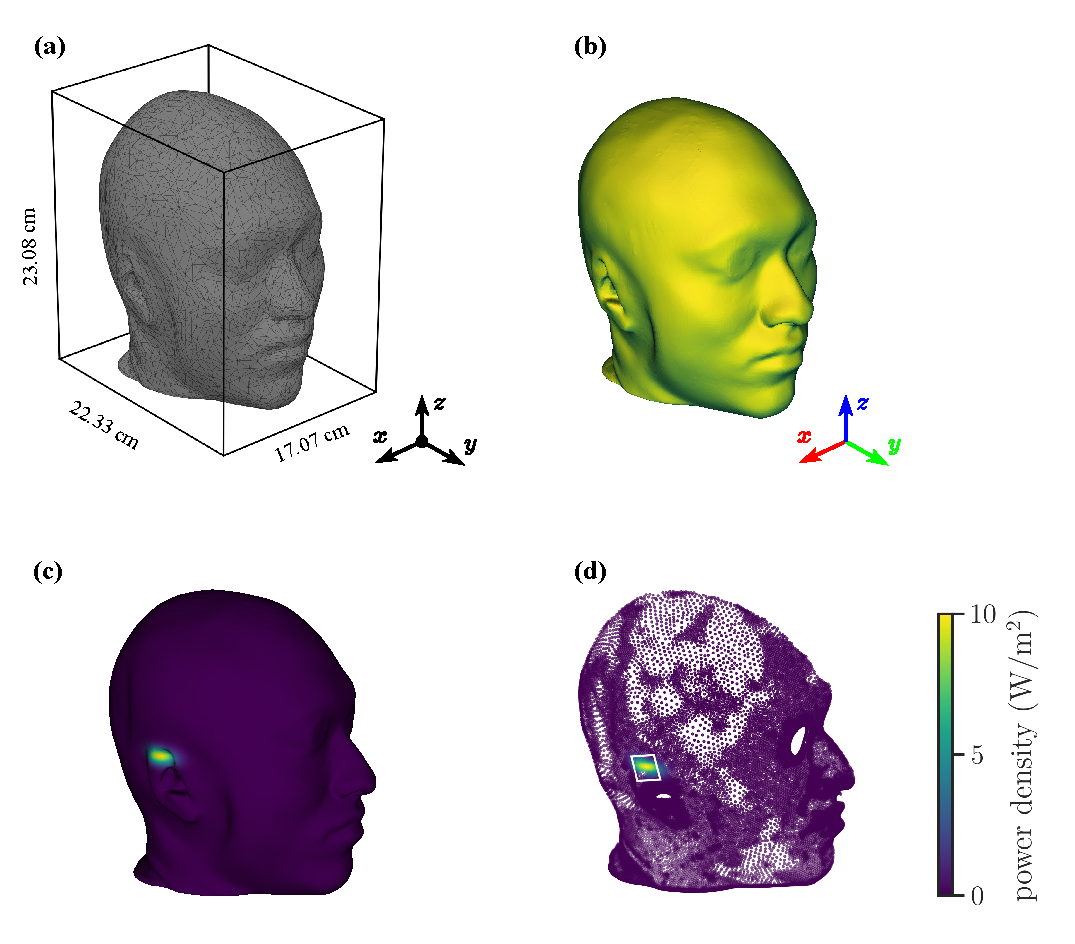
\includegraphics[width=\textwidth]{artwork/head.pdf}
    \caption{Spatial averaging of the power density on the human head model: (a) reconstructed surface of the human head, (b) unit normals directed outward from the surface (represented using red-green-blue values), (c) distribution of the power density in a Gaussian pattern with the peak value located in the upper crus of the right antihelix, (d) position of the square projection of the conformal averaging region on the surface where the spatial averaging of the power density results in a global maximum value.}
    \label{fig:head} 
\end{figure}
